%==============================================================================
% Voorbeeld hogent-article: onderzoeksvoorstel bachproef
%==============================================================================

\documentclass{hogent-article}

\usepackage{lipsum} % Voor vultekst

% Invoegen bibliografiebestand
\addbibresource{references.bib}

% Informatie over de opleiding, het vak en soort opdracht
\studyprogramme{Professionele bachelor toegepaste informatica}
\course{Research Methods}
\assignmenttype{Paper: Onderzoeksvoorstel}
\academicyear{2022-2023}

\title{Automatische bijsturing van het elektriciteitsverbruik van gezinnen met behulp van artificiële intelligentie (AI)}

\author{Jan Tubeeckx}
\email{jan.tubeeckx@student.hogent.be}

\projectrepo{https://github.com/HoGentTIN/rm-2223-paper-rmjantubeeckx}

% Binnen welke specialisatierichting uit 3TI situeert dit onderzoek zich?
% Kies uit deze lijst:
%
%- Mobile \& Enterprise development
% - AI \& Data Engineering
% - Functional \& Business Analysis
% - System \& Network Administrator
% - Mainframe Expert
% - Als het onderzoek niet past binnen een van deze domeinen specifieer je deze
%   zelf
%
\specialisation{Mobile \& Enterprise development}
% Geef hier enkele sleutelwoorden die je onderwerp beschrijven
\keywords{Elektricitetsverbruik, digitale elektriciteitsmeter, AI, distributienet, spreiding}

\begin{document}

\begin{abstract}
  Het doel van dit onderzoek is te achterhalen hoe het elektriciteitsverbruik van gezinnen automatisch kan worden bijgestuurd en gespreid met behulp van artificiële intelligentie (AI) en een mobiele app die verbonden is met een digitale elektriciteitsmeter en een weer API. Door de omschakeling naar hernieuwbare energie wordt volop ingezet op elektrificatie. Dit vraagt enerzijds een modernisering van het distributienetwerk voor elektriciteit, maar  ook de inzet van slimme technologieën, zoals de digitale elektriciteitsmeter. Deze meter kan slim gemaakt worden door er apps mee te verbinden die gezinnen inzicht geven in hun energieverbruik zodat ze dit kunnen bijsturten en spreiden. Hiermee kan het distributienetwerk dan efficiënter gebruikt worden, zodat overdreven investeringen kunnen vermeden worden. \\
  
  In het eerste deel van het onderzoek zal worden nagegaan welke apps er momenteel bestaan en wat hun tekortkomingen zijn. De \textcite{VREG2021} heeft vastgesteld dat het slim maken van digitale elektriciteitsmeters voorlopig niet tot de gewenste gedragsverandering en spreiding van het verbruik van elektriciteit leidt. Het merendeel van deze apps geeft immers enkel op een passieve manier inzicht in het elektriciteitsverbruik en laat de bijsturing ervan over aan de gebruiker. \\
  
  In het tweede deel van dit onderzoek zal daarom een app ontwikkeld worden die met behulp van artificiële intelligentie en een weer API het elektriciteitsverbruik automatisch en dus actief zal bijsturen en spreiden. Meer concreet zal AI worden gebruikt om voorspellingen te doen op basis van historische verbruiksdata die dan gecombineerd worden met weersvoorspellingen die verkregen worden via een weer API. De app zal dan op basis van de gecombineerde voorspellingen een warmtepomp en sanitaire toestellen automatisch gaan in- of uitschakelen. Daarbij zal de gebruiker wel nog steeds de mogelijkheid geboden worden om manueel tussen te komen. \\
  
  Het verwachte resultaat is dat het elektriciteitsverbruik op die manier wel meer gestuurd en gespreid zal worden. Dit zal niet alleen tot een ontlasting van het distributienetwerk voor elektriciteit leiden, maar zal ook de energiekosten voor de gezinnen drukken.
  
\end{abstract}

\tableofcontents

\bigskip

\section{Inleiding}%
\label{sec:inleiding}
Anderhalf miljoen elektrische wagens, massaal veel warmtepompen en zonnepanelen gecombineerd met een toenemende elektrificatie van de industrie en het vrachtvervoer tegen 2030. Dat is de verwachting van de Vlaamse distributienetbeheerder Fluvius \autocite{Verdoodt2022}. De energietransitie die vanuit Europa, België en Vlaanderen wordt aangestuurd, vormt een enorme uitdaging voor de distributienetten voor elektriciteit in Vlaanderen.

\begin{figure}
    \centering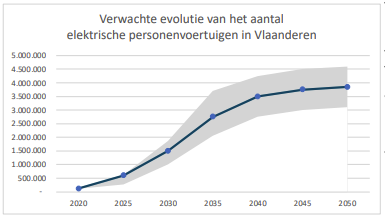
\includegraphics[scale=0.5]{img/Aantal_el_personenvoertuigen}
    \caption{\label{fig:Aantal_el_personenvoertuigen}Verwachte evolutie van het aantal
        elektrische personenvoertuigen in Vlaanderen \autocite{Verdoodt2022}.}
\end{figure}

\begin{figure}
    \centering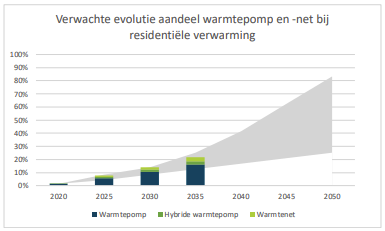
\includegraphics[scale=0.5]{img/Evolutie_Warmtepompen}
    \caption{\label{fig:Evolutie_Warmtepompen}Verwachte evolutie aandeel warmtepomp en -net bij
        residentiële verwarming \autocite{Verdoodt2022}.}
\end{figure}

\begin{figure}
    \centering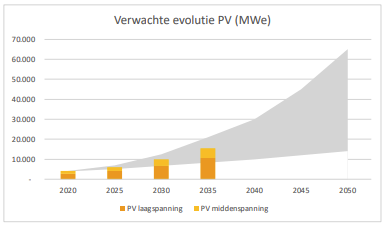
\includegraphics[scale=0.5]{img/Evolutie_PV}
    \caption{\label{fig:Evolutie_PV}Verwachte evolutie PV (MWe) \autocite{Verdoodt2022}.}
\end{figure}

\begin{figure}
    \centering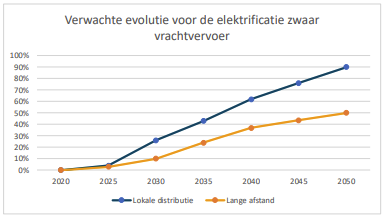
\includegraphics[scale=0.5]{img/El_Vrachtvervoer}
    \caption{\label{fig:El_Vrachtvervoer}Verwachte evolutie voor de elektrificatie zwaar
        vrachtvervoer \autocite{Verdoodt2022}.}
\end{figure}

Om al te hoge investeringen in de distributienetten te vermijden, wordt door Fluvius ingezet op maatregelen die de belasting van het elektriciteitsnet kunnen verminderen en spreiden. Een van die maatregelen is de invoering en verplichting van de digitale elektriciteitsmeter. Tegen juli 2029 moeten alle Belgische huishoudens een digitale meter hebben. Deze digitale meters kunnen via een dongle en een app 'slimmer' gemaakt worden, zodat gezinnen hun elektriciteitsverbruik in detail kunnen opvolgen en bijsturen. Dit zal dan meteen ook een besparing voor hen opleveren. Deze apps vereisen echter steeds een actieve opvolging van de gebruiker. Uit onderzoek is gebleken dat deze actieve bijsturing na verloop van tijd vermindert \autocite{Wemyss2019}. Een enquête van de \textcite{VREG2021} waarin 1.000 Vlaamse gezinnen en 1.500 bedrijven bevraagd werden over hun ervaring en gedrag op de energiemarkt toont zelfs aan dat van de 60\% van de gezinnen met een digitale meter, slechts 8\% hun energieverbruik effectief bijstuurt. Door de invoering van het capaciteitstarief, een andere maatregel waarmee de VREG het elektriciteitsnet hoopt te ontlasten, zal de bijsturing en vooral spreiding van het elektriciteitsverbruik nog belangrijker worden voor gezinnen. Sinds 1 januari 2023 wordt immers een deel van de nettarieven die een gezin via haar elektriciteitsfactuur betaalt ook berekend op het maximale elektriciteitsverbruik. Er wordt dus voortaan ook gekeken naar de maximale capaciteit die de distributienetbeheerders ter beschikking moeten stellen. Bedoeling van het capaciteitstarief is dat gezinnen hun stroomverbruik beter gaan spreiden. Als iedereen op hetzelfde moment veel stroom verbruikt, kan het net overbelast raken. Het gevolg is dat netbedrijven dan extra moeten investeren in zwaardere elektriciteitskabels om die hogere verbruikspieken op te vangen \autocite{Selleslagh2022}.

Daarom wordt binnen Fluvius de vraag gesteld hoe nieuwe technologieën en technieken een oplossing kunnen bieden om gezinnen te helpen bij het spreiden van hun elektriciteitsverbruik. Kunnen apps die het elektriciteitsverbuik monitoren slimmer gemaakt worden zodat ze geen tussenkomst van een gebruiker meer behoeven? Kan bijvoorbeeld artificiële intelligentie (AI) daarbij een oplossing bieden? Om dit na te gaan, zal tijdens dit onderzoek een app ontwikkeld worden die het elektriciteitsverbruik zal aansturen op basis van weersvoorspellingen en historische verbruiksdata.

\bigskip
\bigskip
\bigskip
\bigskip
\bigskip
\bigskip
\bigskip
\bigskip
\bigskip
\bigskip
\bigskip
\bigskip
\bigskip
\bigskip
\bigskip
\bigskip
\bigskip
\bigskip
\bigskip

\section{Literatuurstudie}%
\label{sec:literatuurstudie}

Met een digitale elektriciteitsmeter kunnen gezinnen hun elektriciteitsverbruik makkelijk opvolgen. Dat kan in de eerste plaats gratis via het online energieportaal \href{https://login.fluvius.be/klanten.onmicrosoft.com/b2c_1a_customer_signup_signin/oauth2/v2.0/authorize?client_id=91bb9a0a-f45d-491a-ae0b-43324fbc343a&scope=openid%20profile%20offline_access&redirect_uri=https%3A%2F%2Fmijn.fluvius.be%2Fredirect&client-request-id=90c12c72-7d7b-428b-98fc-5d7956e53a60&response_mode=fragment&response_type=code&x-client-SKU=msal.js.browser&x-client-VER=2.23.0&client_info=1&code_challenge=jz-1E8AwB15UEa352eC_5x6zDtAtwp3Je6jrFVdGKjk&code_challenge_method=S256&nonce=cee3d720-d931-4b13-b0b5-c473169ca6fd&state=eyJpZCI6IjRhM2I3M2NkLTgyZjgtNDFjOC05NzAyLTEwMTNjNjNkNjNhMyIsIm1ldGEiOnsiaW50ZXJhY3Rpb25UeXBlIjoicmVkaXJlY3QifX0%3D}{Mijn Fluvius}. Daarnaast bestaan er ook heel wat gratis of betalende online apps die op de gebruikerspoort van de digitale meter kunnen worden aangesloten om elektriciteitsverbruik op te volgen en de mogelijkheid bieden om andere toestellen aan te sturen. Een overzicht van deze toepassingen vindt men op de website \href{https://maakjemeterslim.be/}{www.maakjemeterslim.be}.

De digitale elektriciteitsmeter heeft twee gebruikerspoorten waar verschillende toestellen aan kunnen worden gekoppeld. Beide gebruikerspoorten zijn complementair en geschikt voor verschillende toepassingen. De P1-poort stuurt de elektriciteitsdata per seconde rechtstreeks uit. Via de ‘snelle’ S1-poort worden ruwe data aan een hoge frequentie ter beschikking gesteld. Beide poorten laten gedetailleerde verbruikersfeedback en sturing van huishoudapparaten toe. Op de gebruikerspoorten (P1 en/of S1) kan een energiebeheersysteem worden aangesloten \autocite{Depuydt2021}. Concreet gaat het om apps, slimme thermostaten of andere toestellen waarmee men elektriciteitsverbruik actief kan beheren. Zo’n toepassingen heten in het jargon ‘HEMS’ (Home Energy Management System) of ‘CEMS’ (Customer Energy Management System). De verbinding tussen het meettoestel en een app gebeurt in de meeste gevallen via een wifiverbinding of 4G.

De bestaande apps bieden allemaal de mogelijkheid om elektriciteitsverbruik in real time op te volgen. In elf gevallen kan dat naast een overzicht op de smartphone, tablet of computer ook via een afzonderlijk beeldscherm op de muur. Het meten van de energiekosten per huishoudtoestel behoort standaard tot verschillende apps, maar geldt ook vaak als een optie. De meeste apps sporen ook sluipverbruik op en bieden gepersonaliseerde tips voor energiebesparing. Sommige apps bieden tenslotte ook de mogelijkheid om het gemeten elektriciteitsverbruik naast weerdata te leggen en op die manier na te gaan hoeveel stroom men verbruikt bij bepaalde weersomstandigheden \autocite{Deman2021}. Het is duidelijk dat al deze apps slechts op een passieve het elektriciteitsverbruik van de gebruiker bijsturen. Het is de gebruiker zelf die op basis van de gevevens die de app hem toont actie kan ondernemen. En hoewel sommige bestaande apps efficiënter dan andere blijken \autocite{Mack2016} en \autocite{Wood2019}, leidt dit zoals reeds eerder werd vermeld, niet altijd tot de gewenste gedragsverandering \autocite{Wemyss2019}, \autocite{Mack2019} en  \autocite{VREG2021}.

Omdat het noodzakelijk is dat gezinnen en bedrijven bewuster en actiever met hun energieverbuik gaan omspringen, wordt binnen Fluvius en ook andere bedrijven gekeken naar nieuwe technologieën en technieken \autocite{Verdoodt2018}. Dit bracht mij op het idee om een app te gaan ontwikkelen die wel actief en dus automatisch het elektriciteitsverbruik kan gaan bijsturen. Omdat er reeds apps bestaan die weerdata gebruiken om het elektriciteitsverbruik onder bepaalde weersomstandigheden in kaart te brengen, lijkt het me zeker mogelijk om weerdata ook als aansturing te gaan gebruiken, samen met de historieken van het elektriciteitsverbruik om dan zo het toekomstig elektriciteitsverbruik en de elektriciteitsproductie te voorspellen \autocite{Guo2022}. Er zijn tal van bestaande gratis weer API's, zoals \href{https://openweathermap.org/api}{Open Weather Map} of \href{https://www.weatherapi.com/}{Weather API} die kunnen geïntegreerd worden in een app. Om de voorspellingen zo accuraat mogelijk te maken, zal gebruik gemaakt worden van het Extreme Gradient Boosting (XGBOOST) algoritme \autocite{Ledmaoui2023}, \autocite{Wang2022} en \autocite{BarreraAnimas2022}. De historische verbruiksdata, de productiedata van de omvormer van de zonnepanelen en de weerdata zullen als input gebruikt worden voor dit algoritme. De data van de digitale elekticiteitsmeter en de omvormer van de zonnepanelen wordt continue uitgelezen met een python script op een Raspberry Pi computer die via het wifi-netwerk verbonden is. Deze data wordt opgelsagen in een NoSQL-databank die speciaal voor time-series ontwikkeld is, nl. InfluxDB \autocite{Balis2017} en  \autocite{Struckov2019}. De app zal tenslotte ontwikkeld worden voor iOS en gebouwd worden met Xcode, SwiftUI en UIKit \autocite{Allardice} en \autocite{Firtman2022}.

De eerste slimme toestellen die via de app zullen worden beheerd zijn zonnepanelen en een warmtepomp \autocite{Uytterhoeven2019}. Door de afschaffing van de virtueel terugdraaiende teller voor eigenaars van zonnepanelen, waarbij de teller van de elektriciteitsmeter terugdraait wanneer meer elektriciteit wordt opgewekt dan verbruikt, kan het verlies van dit voordeel opgevangen door het verbruik van de warmtepomp te laten samenvallen met de productiemomenten van de zonnepanelen \autocite{Selleslagh2021}. Wanneer echter uit de weersverwachtingen blijkt dat er een aanzienlijke elektriciteitsproductie zal zijn, zal de app  mede op basis van historiek van het elektriciteitsverbruik automatisch ook andere toestellen, zoals de vaatwas of wasmachine gaan inschakelen. Om de sanitaire toestellen te kunnen gaan inschakelen, zal in de eerste plaats gekeken worden of deze toestellen van zichzelf reeds slim zijn. Meer concreet zal geverifieerd worden of ze over een Soft Real Time Operating System beschikken (Soft RTOS) en via het wifinetwerk kunnen communiceren met een app. Voor de sanitaire toestellen die niet slim zijn, zal gebruik gemaakt worden van slimme stopcontacten. Daarbij wordt er tussen het klassieke stopcontact en de stekker van het toestel een apparaat geplaatst, waardoor een toestel op een eenvoudige manier slim kan gemaakt worden \autocite{Jong2020}.

% Refereren naar de literatuur kan met:
% \autocite{BIBTEXKEY} -> (Auteur, jaartal)
% \textcite{BIBTEXKEY} -> Auteur (jaartal)
\newpage \pagebreak \cleardoublepage
\section{Methodologie}%
\label{sec:methodologie}

Het onderzoek zal aangevat worden met een studie van bestaande apps die kunnen verbonden worden met een digitale elektriciteitsmeter en waarmee elektricteitsverbruik kan opgevolgd en beheerd worden. Er bestaan heel wat gratis apps die elektriciteitsverbruik kunnen visualiseren en aansturen. Bedoeling is om een aantal van deze apps uitvoerig te gaan bestuderen. Wat zijn de functies die ze bieden. Hoe visualiseren deze apps het elektriciteitsverbruik en op welke manier kan het verbruik bijgestuurd worden. Door deze studie kan worden aangetoond dat de meeste van de apps om elektriciteitsverbruik te beheren louter passief werken en steeds een actie van de gebruiker vereisen.

In het tweede deel van het onderzoek zal een app ontwikkeld worden die met behulp van artificiële intelligentie historische verbruiksdata en weersvoorspellingen zal gebruiken om het elektriciteitsverbruik automatisch aan te sturen en te beheren. Vooreerst zal de data van de digitale elektriciteitsmeter worden uitgelezen met behulp van een Raspberry Pi 2GB. De uitgelezen data zal worden opgeslagen in een Azure databank. Wanneer voldoende verbruiksdata verzameld is, zal artificiële intelligentie gebruikt worden om toekomstig elektriciteitsverbruik te voorspellen. Daarvoor zal in eerste instantie gekeken worden naar een bestaand AI platform zoals Azure AI van Microsoft. Om de voorspelling nog acurater te kunnen maken, zal de historische verbruiksdata gecombineerd worden met weersvoorspellingen van een open source weer API. De voorspellingen zullen vervolgens gebruikt worden om slimme of slim gemaakte toestellen automatisch te gaan in- of uitschakelen. Om dit alles inzichtelijk te maken voor de gebruiker zal een mobiele applicatie in IOS ontwikkeld worden. Via deze mobiele applicatie zal de gebruiker ook de mogelijkheid hebben om handmatig bij te sturen indien hij of zij dit wenst.

Nadat de app ontwikkeld is, zal een selectie worden gemaakt van welke elektrische toestellen de app zal aansturen. Er zal nagegaan worden met welke toestellen het meeste elektriciteit bespaard kan worden door ze met weersvoorspellingen aan te sturen. Verder zal ook bepaald worden op welke manier de gekozen toestellen slim kunnen gemaakt worden. Zijn de toestellen reeds slim van zichzelf, zoals bijvoorbeeld sommige zonnepanelen dat zijn, of moeten de toestellen slim gemaakt worden? Een optie daarbij is het gebruik van slimme stopcontacten. Daarbij kan er tussen het klassieke stopcontact en de stekker van het toestel een apparaat geplaatst worden, waardoor een klassiek stopcontact zonder ingrijpende werken slim kan gemaakt worden.

%Om na te gaan of de app een elektriciteitsbesparing oplevert, zullen een aantal testgebruiker de app gedurende een maand testen. Om de werking van de app te kunnen testen zullen vijf testgebruikers geselecteerd worden. Zij zullen de app gedurende een maand gebruiken. In de eerste plaats zal de testgebruikers gevraagd worden om elke dag na te gaan of en wanneer de verbonden slimme toestellen door de app aangestuurd werden. In de app zal namelijk steeds een overzicht van de in- en afschakelmomenten van de verschillende toestellen beschikbaar zijn. Daarnaast zullen de testgebruikers ook gevraagd worden om een manuele bijsturing te noteren en kort de reden hiervan te vermelden. Telkens wanneer de app een verbonden toestel niet correct in- of uitschakelt, kan de gebruiker tussenkomen en het desbtreffende toestel zelf in- of uitschakelen. Na afloop van deze onderzoeksfase zullen vijf testgebruikers, waaronder de onderzoeker zelf, de app gedurende een maand getest hebben.

Na de testperiode zal worden geverifieerd in welke mate de app de ermee verbonden apparaten correct heeft in- en uitgeschakeld. Meer concreet zal worden nagegaan hoe vaak de door de app aangestuurde toestellen correct werden in- of uitgeschakeld. Daarvoor zullen de door de app geregistreerde gegevens vergeleken worden met de door de testgebruikers genoteerde manuele tussenkomsten. Ook zal de testgebruikers een vragenlijst worden voorgelegd, waarin naar hun ervaringen met het gebruik van de app gepeild wordt. Zo zal er gevraagd worden of de app op de juiste momenten de ermee verbonden toestellen in- en uitschakelde. Er zal een verslag worden opgemaakt waarin per testgebruiker en per toestel de manuele bijsturingen in kaart worden gebracht. Hieraan zullen ook de antwoorden op de vragenlijst worden toegevoegd, zodat per testgebruiker een conclusie kan getrokken worden.

\section{Verwachte resultaten}%
\label{sec:verwachte-resultaten}

De verwachting is dat na afloop van dit onderzoek de zelfconsumptie van de testdeelnemers verhoogd is en het elektriciteitsverbruik meer gespreid wordt. Om hieruit ook werkelijk een financieel voordeel te halen, zal de minstens 50\% zelfverbruik moeten behaald worden \autocite{Selleslagh2021}. Als naast de warmtepomp ook een wasmachine, vaatwasmachine en een elektrisch voertuig kunnen worden aangesloten op de ontwikkelde app, zal dit percentage zeker behaald kunnen worden. 

Omdat ook piekverbruiken moeten vermeden worden omwille van het capaciteitstarief, zal de app enkel toestellen inschakelen indien de elektriciteit die door de zonnepanelen gegenereerd wordt toereikend is om aan het gecombineerde verbruik te voldoen. Op basis van de weersverwachtingen zal de app gaan inschatten of de productie voldoende lang kan gegarandeerd worden. Zo zullen meerdere toestellen tegelijkertijd kunnen worden ingeschakeld zonder een verbruikspiek te veroorzaken. Omgekeerd zal de app er ook voor zorgen dat op dagelijkse piekmomenten sommige toestellen worden uitgeschakeld, indien er onvoldoende elektriciteit wordt opgewekt door de zonnepanelen. Zo zal de warmtepomp uitgeschakeld worden op het moment dat al veel andere apparaten aan het werk zijn. Verwacht wordt dat de app de piekverbruiken zo automatisch tot een minimum zal herleiden, waardoor de nettarieven en dus de elektriciteitsfactuur voor gezinnen kan verlaagd worden.
\autocite{Balakumar2023} \autocite{Gozuoglu2024}  \autocite{Tziolis2024}  \autocite{Guerra2024}  \autocite{Bozlak2024}  \autocite{Kim2023} \autocite{Hoseinpour2024}  \autocite{Volta2023} \autocite{Konsman2023} \autocite{Fluvius2023}

%\section{Discussie, conclusie}%
%\label{sec:discussie-conclusie}

\bigskip
\bigskip
\bigskip
\bigskip
\bigskip
\bigskip
\bigskip
\bigskip
\bigskip
\bigskip
\bigskip
\bigskip
\bigskip
\bigskip
\bigskip
\bigskip
\bigskip
\bigskip
\bigskip


%------------------------------------------------------------------------------
% Referentielijst
%------------------------------------------------------------------------------
% bibliografie.bib voorkomen. Gebruik JabRef om je bibliografie bij te
% houden.

\printbibliography[heading=bibintoc]

\end{document}